\documentclass[letterpaper, 12pt, oneside]{article}%especificaciones del documento
\usepackage{amsmath}%paquete para escribir expresiones matemámaticas
\usepackage{graphicx}%paquete para poder incluír imagenes en el documento
\usepackage{xcolor} %paquete de LaTex para poder poner otro texto
\graphicspath{{Imagenes/}}%directorio de la imagen, este lo cambian por el directorio en el que ustedes guardaron su imagen 1.png
\usepackage[utf8]{inputenc} %para poder poner acentos0

	\title{\Huge Taller de Herramientas Computacionales}
	%\title{\Huge \colorbox{magenta}{Taller de Herramientas computacionales}} %De esta forma con colorbox pone el texto dentro de una "caja" de color.
	\author{Josué Artemio Hernández Rodríguez}%autor del escrito
	\date{10/01/19}%fecha del escrito

\begin{document}%inicia el documento
\maketitle
%\vfill %Para rellenar el espacio y colocar hasta abajo de la pagina el siguiente texto, imagen.
\begin{center}%inicia centrado
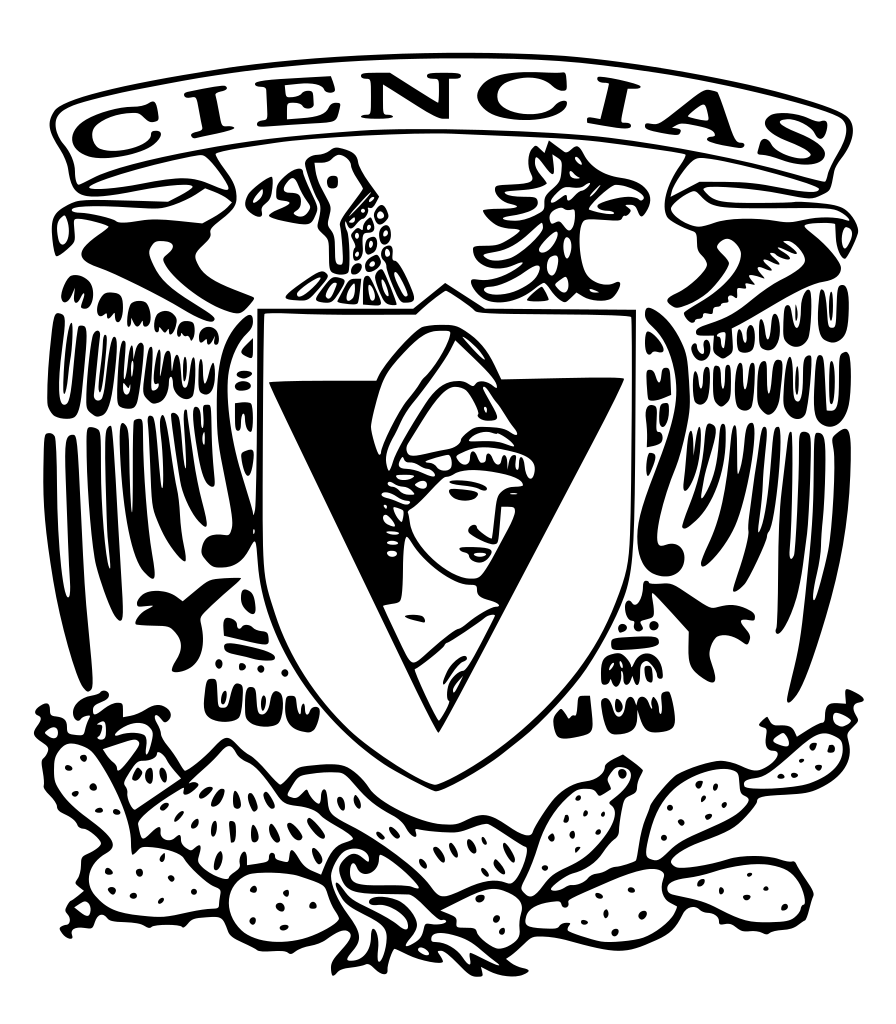
\includegraphics[scale=0.2]{2.png}%del lado izquierdo se muestra el tamaño de la imagen, del derecho se escribe el nombre de la imagen a incluir en el texto
\end{center}%termina el centrado para la imagen
\newpage%crea una nueva página

\title{\Huge Resolviendo un problema con python\\}%titulo2 \\ sirven para saltar una linea.

Lo que vimos en clase fue:%letras de color azul
\begin{enumerate}%Inicio de númeración para enlistar las cosas vistas en clase.
	\item Algunos conceptos y software utilizado en clase%item sirve enlistar el elemento, este es el primer elemento enumerado.
		\begin{enumerate}
			\item idle: Es un IDE, entornno de desarrollo integrado, dicho de otro modo es un editor especializado que tiene una forma de comunicación con el interprete, una de sus ventajas es que tiene herramienta de depuracion de errores
			\item shell, es un interprete de comandos, forma parte de las herramientas de idle
			\item En python, el símbolo de "gato" se utiliza para realizar comentarios en el código
		\end{enumerate}
	
	\item Comandos de Bash y python %Segundo elemento enumerado.
	\begin{itemize}%comienza el enlistado pero itemize a diferencia de enumerate enlista sin un orden secuencial (es decir no utiliza números, ni letras)
		\item dnf install python-tools : instala los paquetes necesarios para usar idle
		\item python + doble Tab , muestra los archivos que inician con la palabra python
		\item 1/2 Da como resultado 0.0 porque esta dividiendo partes enteras, lo correctoes usar 1.0/2 o al revez, 1/2.0
		\item print muestra en pantalla lo que se deseé
		
				
	\end{itemize}%finaliza enlistado con itemize
	
	\item \textbf{Tarea}
	\\
	Hacer el problema que buscamos en codigo de python
		
	
\end{enumerate}%finaliza el enlistado principal
	


\end{document}%termina el documento